\chapter{Introducción específica} % Main chapter title

\label{Chapter2}

%----------------------------------------------------------------------------------------
%	SECTION 1
%----------------------------------------------------------------------------------------
Este capítulo presenta los principales componentes tecnológicos que conforman el sistema desarrollado. Se describe la arquitectura general, los dispositivos seleccionados y las tecnologías de comunicación utilizadas. También se exponen los escenarios de uso previstos y las posibles aplicaciones prácticas de la solución.

\section{Arquitectura general del sistema}
\label{sec:Arquitectura general del sistema}

El sistema se organiza en torno a tres componentes principales: nodos sensores distribuidos, mecanismos de transmisión y una plataforma web de consulta. Esta estructura permite recolectar datos ambientales para su posterior procesamiento en una infraestructura centralizada. La figura \ref{fig:2-1-diagrama} ilustra de forma esquemática la interconexión entre estos elementos.

\begin{figure}[h]
    \centering
    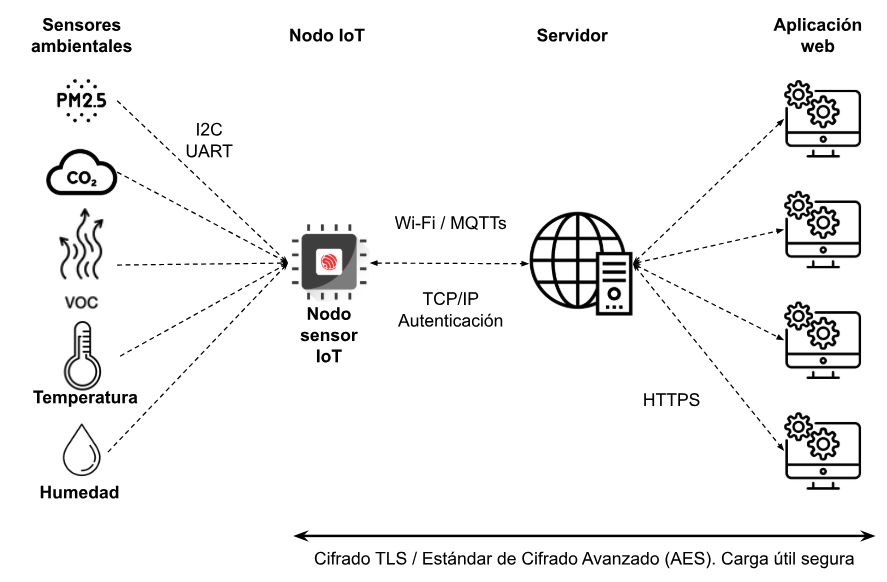
\includegraphics[width=0.85\linewidth]{Figures/2_1-diagrama.png}
    \caption{Diagrama de bloques del sistema de monitoreo de calidad de aire.}
    \label{fig:2-1-diagrama}
\end{figure}

Cada unidad recolectora utiliza el microcontrolador \texttt{ESP32 Heltec V3} \cite{heltec:v3} para la gestión de sensores y la comunicación inalámbrica. El nodo integra sensores específicos para medir material particulado, gases contaminantes y variables climáticas.

La transmisión de datos se realiza hacia un servidor central mediante el protocolo \textit{MQTT} (del inglés, \textit{Message Queuing Telemetry Transport}) sobre una red \textit{Wi-Fi}. Finalmente, una plataforma web desarrollada con herramientas modernas permite la visualización de la información en tiempo real.

%----------------------------------------------------------------------------------------

\section{Dispositivos IoT y sensores seleccionados}

Para el desarrollo del sistema se optó por el microcontrolador \texttt{ESP32 Heltec V3} como unidad cental de los nodos. Esta placa integra un procesador de docle núcleo y conectividad \textit{Wi-Fi} nativa. La elección responde a su bajo consumo energético y la compatibilidad con múltiples interfaces de comunicación digital como \texttt{I2C} y \texttt{UART}.

Se seleccionaron sensores ambientales con un equilibrio entre costo y confiabilidad técnica. Estos compoenentes permiten caracterizar la calidad del aire mediante la medición de partículas y gases. Todos los dispositivos elegidos emplean protocolos de comunicación digital para asegurar la integridad de las señales frente a interferencias.

Los sensores principales que integran la solución son:

\begin{itemize}
    \item \texttt{PMS7003} \cite{plantower:pms7003}: sensor óptico que utiliza la dispersión láser para medir material particulado ($PM_{2.5}$ y $PM_{10}$).
    \item \texttt{CJMCU-4541}: módulo multigas para la detección de monóxido de carbono, dióxido de nitrógeno y amoníaco.
    \item \texttt{SCD40} \cite{sensirion:scd40}: sensor fotoacústico para la medición de $CO_2$, temperatura y humedad relativa.
    \item \texttt{SGP30} \cite{sensirion:sgp30}: sensor de membrana de metal-óxido para la detección de compuestos orgánicos volátiles (\textit{VOCs}).
\end{itemize}

La tabla \ref{tab:sensores} presenta un resumen de los sensores seleccionados, incluidas las variables medidas y sus protocolos de comunicación:

\begin{table}[h]
    \centering
    \caption[Resumen de sensores utilizados]{Sensores seleccionados para el sistema SMCA y sus principales características.}
    \label{tab:sensores}
    \begin{tabular}{p{3.5cm} p{5.5cm} p{2.5cm}}
        \toprule
        \textbf{Sensor} & \textbf{Variable medida} & \textbf{Comunicación} \\
        \midrule
        PMS7003 & PM$_{2.5}$, PM$_{10}$ & UART  \\
        CJMCU-4541 & NO$_2$, CO, NH$_3$ & I2C \\
        SCD40 & CO$_2$, temperatura, humedad & I2C \\
        SGP30 & VOCs & I2C \\
        \bottomrule
    \end{tabular}
\end{table}

%----------------------------------------------------------------------------------------

\section{Tecnologías de comunicación utilizadas}

El sistema emplea una red \textit{wi-Fi} para la tansmisión de datos desde los nodos sensores hacia el servidor central. Esta tecnología permite el despliegue de los dispositivos en entornos con infraestructura de red preexistente. El esquema de comunicación se basa en el protocolo \textit{MQTT} con una capa de seguridad adicional.

\textit{MQTT} se caracteriza por su bajo consumo de ancho de banda y su eficiencia en redes inanlámbricas. El protocolo utiliza un modelo de publicación y suscripción que facilita la gestión de múltiples nodos de forma simultánea. Esta arquitectura resulta adecuada para aplicaciones de monitoreo ambiental donde se requiere un flujo de datos constante y ligero.

La segurdad en la transmisión se garantiza mediante el uso de certificados \textit{TLS}. Este mecanismo asegura la autenticación de los nodos emisores y la confidencialidad de la información. La integración de \textit{TLS} protege el sistema frete a posibles ataques de interceptación en la red.

%----------------------------------------------------------------------------------------
\section{Plataforma web para visualización}

El sistema cuenta con una aplicación web diseñada para asegurar una experiencia fluida en diversos dispositivos. Se seleccionó la biblioteca \texttt{React} para el desarrollo del \textit{frontend} (del inglés, capa de presentación). Esta arquitectura se basa en el modelo de \textit{Single Page Application} (del inglés, aplicación de una sola página).

Esta tecnología permite una navegación eficiente y evita la recarga total del navegador ante cada interacción. La plataforma integra un sistema de gestión de usuarios con diferentes niveles de acceso. Se implementó un panel de control o \textit{dashboard} para la visualización general de los datos ambientales.

La aplicación dispone de menús específicos para la administración de zonas y dispositivos. Asimismo, se habilitó una vista de invitado para la consulta pública de datos sin necesidad de autenticación. El sistema consume servicios de una \textit{API RESTful} (del inglés, \textit{Representational State Transfer}) para obtener información del \textit{backend}.

La persistencia de los datos se realiza en una base de datos no estructurada \texttt{MongoDB}. La seguridad de la aplicación web se garantiza mediante protocolos de cifrado y un esquema de autenticación por roles. Esta estructura modular facilita el mantenimiento y la escalabilidad del ecosistema tecnológico.

%----------------------------------------------------------------------------------------
\section{Escenarios de uso y posibles aplicaciones}

El sistema constituye una herramienta flexible y adaptable a diversos entornos urbanos e industriales. Su arquitectura modular y la interfaz multiusuario permiten su implementación en contextos con distintos niveles de infraestructura y necesidades de monitoreo. Los escenarios de uso más relevantes se detallan a continuación:

\begin{itemize}
    \item Instituciones educativas: permite el monitoreo de la calidad del aire en aulas, patios y entornos próximos a fuentes de contaminación. La información asiste a los equipos directivos en la toma de decisiones sobre ventilación o actividades al aire libre.
    \item Zonas industriales o logísticas: acilita el seguimiento continuo de concentraciones de material particulado y gases en áreas expuestas a emisiones. El sistema ayuda a anticipar situaciones de riesgo y respalda auditorías ambientales.
    \item Gobiernos locales: permite el despliegue de nodos en espacios públicos para generar mapas ambientales dinámicos. Estos datos alimentan procesos de decisión en políticas de transporte, salud y urbanismo.
    \item Organizaciones comunitarias o ambientales: omenta el empoderamiento ciudadano mediante el acceso abierto a datos ambientales. La plataforma identifica zonas críticas y genera alertas tempranas ante condiciones adversas.
\end{itemize}

El sistema contempla tres perfiles de usuarios para su operación:

\begin{itemize}
    \item Administrador general: gestiona organizaciones, zonas y usuarios con acceso completo a todas las funcionalidades.
    \item Supervisor: monitorea dispositivos asignados a una o más zonas, visualiza datos y exporta reportes.
    \item Usuario público: accede a la información de los nodos marcados como públicos sin necesidad de autenticación.
\end{itemize}

Un ejemplo de aplicación práctica ocurre en una escuela ubicada en una zona de alta circulación vehicular. El equipo directivo visualiza los niveles de $PM_{2.5}$ y $CO_2$ durante la jornada escolar a través del panel web. Ante valores elevados, se decide suspender actividades al aire libre y reforzar la ventilación en las aulas. Este escenario demuestra cómo el sistema permite tomar decisiones informadas con base en datos obtenidos en tiempo casi real.